\newpage
\section{Theoretical Background}

\subsection{Introduction to Quadrotor Systems}
A quadcopter, also frequently referred to as a quadrotor, is a type of multirotor helicopter or rotary-wing Unmanned Aerial Vehicle (UAV) that utilizes four rotors to achieve flight \parencite{luukkonen_modelling_2011}. These rotors are typically directed upwards and arranged in a square formation, with each rotor positioned at an equal distance from the center of mass. In this configuration, the four actuators are generally equally spaced by 90° from one another \parencite{idrissi_review_2022}.

\subsubsection{Historical Context}
The origins of quadrotor technology date back to 1907, when the Breguet brothers constructed the Gyroplane No. 1 \cref{fig:gyroplane} . While this marked one of the first manned helicopter flights, it was not a free flight; the machine lacked inherent stability and a proper control mechanism, requiring it to be tethered to the ground \parencite{ghazbi_quadrotors_2016}.

\begin{figure}[h]
    \caption{Gyroplane No. 1 by the Breguet brothers} 
    \label{fig:gyroplane}
    \centering
    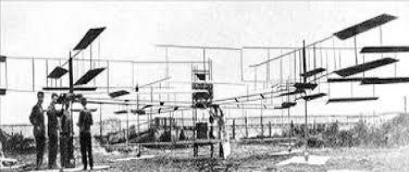
\includegraphics[width=0.8\linewidth]{img/Gyroplane.png}
\end{figure}

The transition to modern UAVs occurred in the late 1990s. A pivotal moment was the 1999 release of the Draganflyer I \cref{fig:dragan}, the first camera-equipped quadrotor to achieve mass production. This shifted quadrotor technology from a laboratory curiosity to a viable commercial product \parencite{karahan2025development}.

\begin{figure}[h]
    \caption{The Draganflyer I} 
    \label{fig:dragan}
    \centering
    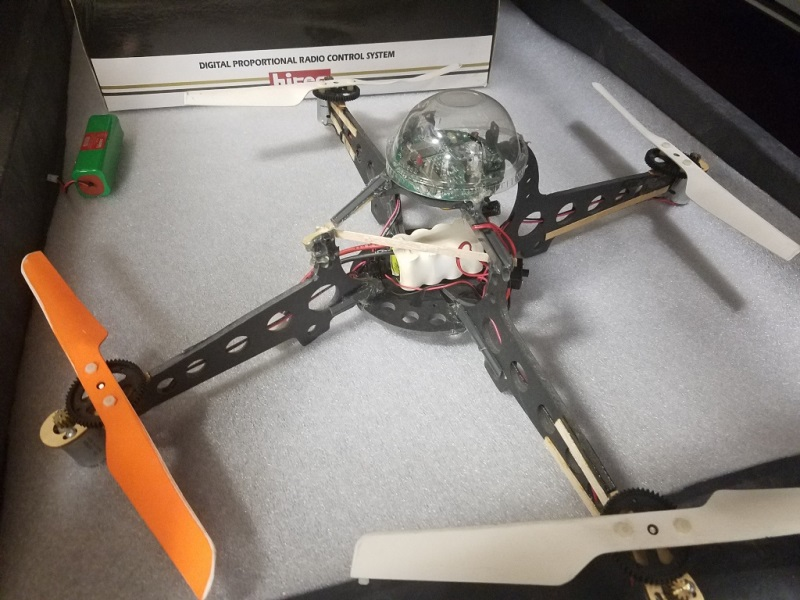
\includegraphics[width=0.8\linewidth]{img/dragan.jpg}
\end{figure}

\subsubsection{Modern Applications}

Since 2010, advancements in micro-electronics and control theory have expanded the use of quadrotors across various sectors:

\begin{itemize}
    \item Public Safety: Search and rescue, firefighting, and border surveillance.
    \item Agriculture: Precision seeding, chemical spraying, and crop monitoring.
    \item Commercial: Last-mile delivery and high-end cinematography.
\end{itemize}

\subsection{Flight Dynamics and Principles of Operation}

A quadcopter is an under-actuated system, meaning it must manage six degrees of freedom (6DOF) \cref{fig:body}, three translational and three rotational—using only four control inputs (the angular velocities of the rotors).

\begin{figure}
    \caption{The inertial and body frames of a quadcopter}
    \label{fig:body}
    \centering
    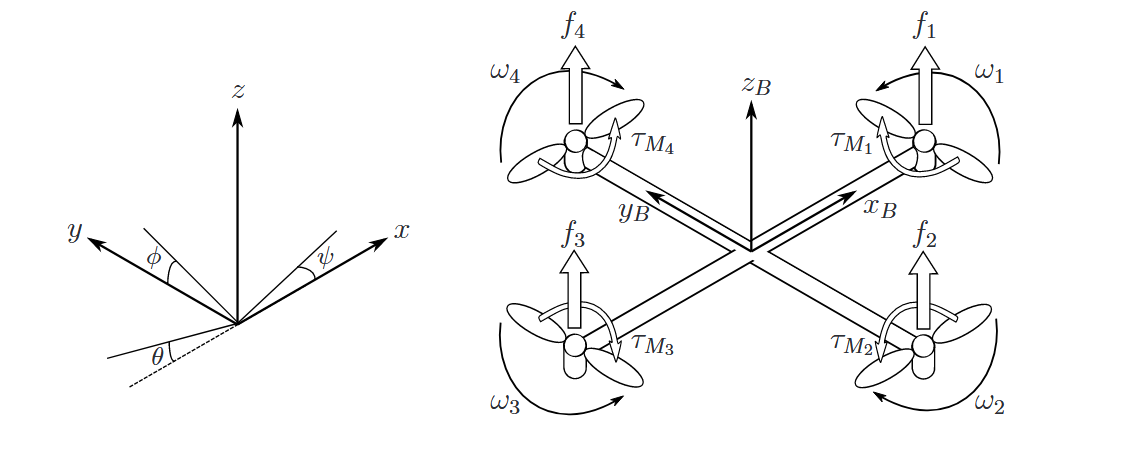
\includegraphics[width=0.8\linewidth]{img/6DOF.png}
\end{figure}

\subsubsection{Torque Cancellation and Configuration}

The fundamental principle of quadcopter stability relies on torque cancellation. To maintain a stable orientation, two motors rotate clockwise (CW) while the adjacent pair rotates counter-clockwise (CCW). This arrangement ensures that the net moment about the center of mass is zero; without this pair-wise opposition, the drone would rotate uncontrollably around its vertical axis. Quadcopters typically use either a "plus (+)" or "cross (x)" configuration, with the cross configuration being more common due to its superior stability \parencite{idrissi_review_2022}.

\subsubsection{Control Inputs}

The absolute linear position of the quadcopter is defined in the inertial frame axes ($[x,y,z]^T$). The attitude, i.e. the angular position, is defined in the inertial frame with three Euler angles ($[\phi, \theta, \psi]^T$), which represent pitch angle, roll angle and yaw angle(figure 3).

Every change in position or attitude is achieved by varying the individual angular velocities ($\omega_i$) of the four rotors:

\begin{itemize}
    \item Thrust ($T$): Simultaneously increasing all rotor speeds causes the vehicle to ascend. The force generated by rotor $i$ is $f_i = k\omega_i^2$, where $k$ is the lift constant. Total thrust is defined as $T = k\sum_{i=1}^4\omega_i^2$.
    \item Yaw ($\tau_\psi$): Rotating the drone around the vertical axis is achieved by creating a torque imbalance between the CW and CCW pairs: $\tau_\psi = b (\omega_1^2 - \omega_2^2 + \omega_3^2 - \omega_4^2)$, where $b$ is the drag constant.
    \item Roll ($\tau_\phi$) and Pitch ($\tau_\theta$): These are achieved by creating a speed differential between opposite rotors. For a distance $l$ from the center of mass:
        \begin{itemize}
            \item $\tau_\phi = l k (-\omega_2^2 + \omega_4^2)$
            \item  $\tau_\theta = l k (-\omega_1^2 + \omega_3^2)$
        \end{itemize}
\end{itemize}

\subsubsection{Mathematical Modeling}

The quadcopter is modeled as a rigid body using **Newton-Euler equations**. The acceleration in the inertial frame $[x,y,z]^T$ is governed by gravity ($g$) and the orientation of the thrust vector:

$$\begin{bmatrix} \ddot{x} \\ \ddot{y} \\ \ddot{z} \end{bmatrix} = \begin{bmatrix} 0 \\ 0 \\ -g \end{bmatrix} + \frac{T}{m} \begin{bmatrix} \cos\psi \sin\theta \cos\phi + \sin\psi \sin\phi \\ \sin\psi \sin\theta \cos\phi - \cos\psi \sin\phi \\ \cos\theta \cos\phi \end{bmatrix}$$

In the body-fixed frame, the angular acceleration is influenced by the external torque ($\tau$), inertia matrix ($I$), and gyroscopic effects:

$$\begin{bmatrix} \dot{p} \\ \dot{q} \\ \dot{r} \end{bmatrix} = \begin{bmatrix} (I_{yy} - I_{zz})qr/I_{xx} \\ (I_{zz} - I_{xx})pr/I_{yy} \\ (I_{xx} - I_{yy})pq/I_{zz} \end{bmatrix} + \begin{bmatrix} \tau_\phi/I_{xx} \\ \tau_\theta/I_{yy} \\ \tau_\psi/I_{zz} \end{bmatrix}$$


\subsection{Pilot Interface and Control Systems}

The First-Person View (FPV) experience is defined by the synchronization between the pilot's inputs and the drone's visual feedback. An FPV drone can be controlled with a traditional remote controller or with a Motion Controller. A Motion Controller allows they user to maneuver the drone using hand gestures which is easy and convenient. The FPV Goggles is a also used for the FPV Drone. It’s the defining factor for the FPV Drone. It connects to the drone’s camera so that the camera user can have full vision of the drone’s camera \parencite{usama2021fpv}.

\subsubsection{Radio Transmission and Stick Modes}

Modern FPV controllers utilize two primary stick configurations. The critical difference between an FPV transmitter and a standard gaming controller is the throttle axis, which lacks a spring-return mechanism to allow for precise altitude maintenance \cref{fig:control}.

\begin{figure}
    \caption{Transmitter(Left) and  Gamepad(Right)}
    \label{fig:control}
    \centering
    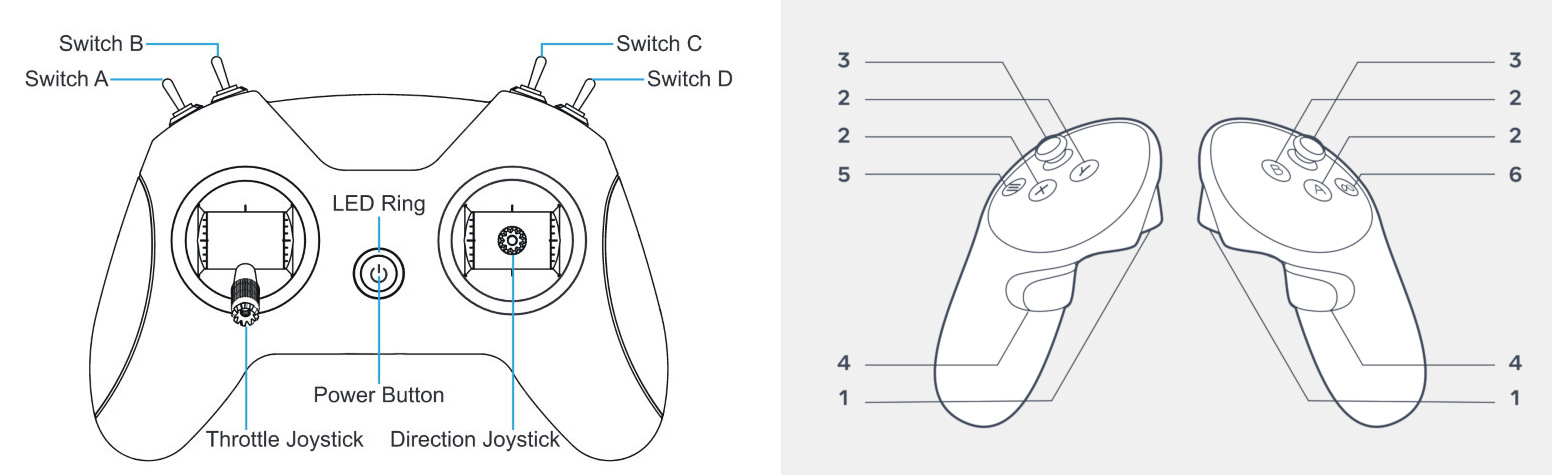
\includegraphics[width=0.8\linewidth]{img/control.jpg}
\end{figure}

The industry standardizes these controls into two primary layouts \cref{fig:modes}:

\begin{itemize}
    \item Mode 1 (Japanese Hand): Predominantly used in Japan and parts of Europe. The throttle is located on the right gimbal.
    \item Mode 2 (American Hand): The global standard for FPV. The throttle is located on the left gimbal, which most pilots find more intuitive for separating altitude from directional pitch.
\end{itemize}

\begin{table}[h]
\label{fig:modes}
\centering
\begin{tabular}{|l|l|l|l|l|}
\hline
Mode & Left Stick (Vertical) & Left Stick (Horizontal) & Right Stick (Vertical) & Right Stick (Horizontal) \\ \hline
Mode 1 & Pitch & Yaw & Throttle & Roll \\ \hline
Mode 2 & Throttle & Yaw & Pitch & Roll \\ \hline
\end{tabular}
\end{table}

From a signal processing perspective, the flight controller differentiates between the unipolar throttle and the bipolar command sticks, \cref{fig:mode2}:

\begin{itemize}
    \item Throttle ($T$): Mapped to a range of $[0, 1]$.
    \item Roll, Pitch, and Yaw ($\phi, \theta, \psi$): Mapped to a range of $[-1, 1]$.
\end{itemize}

\begin{figure}
    \caption{Mode 2 control system}
    \label{fig:mode2}
    \centering
    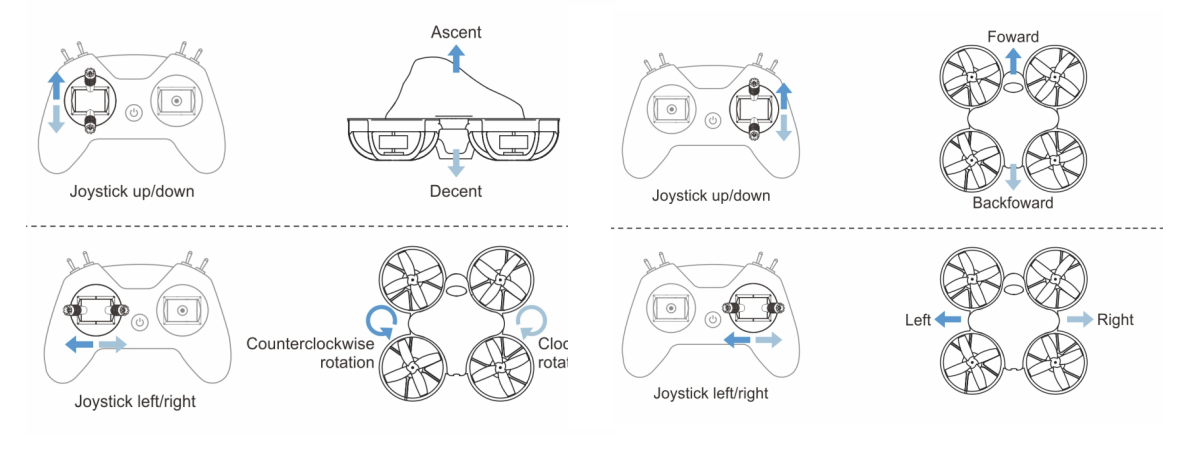
\includegraphics[width=0.8\linewidth]{img/drone.png}
\end{figure}

\subsubsection{Flight Modes}

FPV drones generally operate across two flight logic modes.

\begin{itemize}
    \item Self-Leveling (Angle/Normal Mode): The onboard flight controller uses accelerometers to automatically return the drone to a level horizon when the sticks are centered. This is ideal for beginners but limits maneuverability.
    \item Acrobat (Manual Mode): The controller only uses gyroscopes to maintain the current angular rate. If the pilot moves the stick and returns it to center, the drone maintains its current tilted orientation. This allows for flips and rolls but requires constant manual correction.
\end{itemize}

Although you can use a traditional remote controller to control an FPV quadrotor. There are still a difference on the trottle control in the modern FPV controllers. Take the BetaFPV's LiteRadio 2 SE Radio Transmitter as an example.

\subsubsection{Visual Feedback (FPV Goggles)}

FPV goggles provide the pilot with a low-latency video feed, effectively placing them "inside the cockpit." Beyond the video feed, an On-Screen Display (OSD) provides critical telemetry data, including battery voltage, signal strength (RSSI), and flight time \cref{fig:goggles}.

\begin{figure}
    \caption{goggles interface}
    \label{fig:goggles}
    \centering
    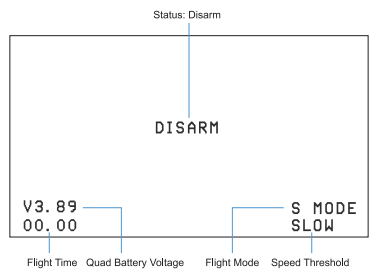
\includegraphics[width=0.8\linewidth]{img/goggles.png}
\end{figure}

\subsection{Implementation of Drone Physics: A Case Study of Yue’s Ultimate Drone}

This section examines the flight dynamics and control implementation found in the "Yue’s Ultimate Drone" \cref{fig:yue} physics model. The system architecture separates pilot input normalization from the underlying Proportional-Derivative (PD) control loops.

\begin{figure}
    \caption{Yue's Ultimate Drone}
    \label{fig:yue}
    \centering
    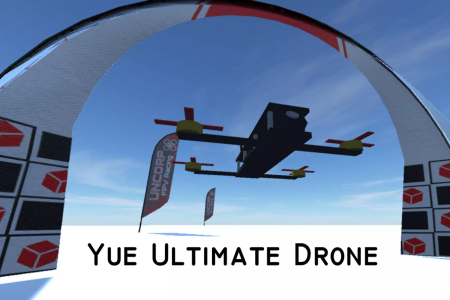
\includegraphics[width=0.8\linewidth]{img/yue.png}
\end{figure}

\subsubsection{Control Input and Joystick Shaping}

The flight controller distinguishes between unipolar throttle inputs and bipolar command sticks (Roll, Pitch, and Yaw):

\begin{itemize}
    \item Throttle ($T$): Mapped to a normalized range of $[0, 1]$.
    \item Attitude Commands ($\theta, \phi, \psi$): Mapped to a range of $[-1, 1]$.
\end{itemize}

To refine the pilot's control over the aircraft, the system utilizes a non-linear control curve for joystick calculation. As Lovesay (2003) observes, a good quality force tracking controller has a linear output, with joystick force directly proportional to sight velocity, but many systems shape the joystick voltage output, to achieve fine control and greater tracking accuracy as the joystick output approaches zero, whilst retaining the same maximum output capability.

In this implementation, "shaping" is achieved by combining proportional ($p$) and exponential ($e$) components to calculate the target angular rate ($\tau$) from the raw angular rate ($u$):

$$\tau = p \cdot u + e \cdot \text{sgn}(u) \cdot u^{2}$$

The specific rates for the rotational axes are calculated as follows:

\begin{itemize}
    \item Yaw Rate ($\tau_\psi$): $\tau_\psi = p \cdot u_\psi + e \cdot \text{sgn}(u_\psi) \cdot u_\psi^{2}$
    \item Roll Rate ($\tau_\phi$): $\tau_\phi = p \cdot u_\phi + e \cdot \text{sgn}(u_\phi) \cdot u_\phi^{2}$
    \item Pitch Rate ($\tau_\theta$): $\tau_\theta = p \cdot u_\theta + e \cdot \text{sgn}(u_\theta) \cdot u_\theta^{2}$
\end{itemize}

The raw gamepad throttle $u_T \in [-1, 1]$ is normalized to a linear thrust scalar:

$$T = \frac{u_T + 1}{2}$$

\subsection{Flight Modes and Orientation Logic}

Since the Unity engine utilizes the FixedUpdate method for physics calculations, the drone's target orientation is updated discretely at every physics timestep ($\Delta t$).

In Acro mode, the joystick inputs command the angular rate of change. The drone's target orientation $q_{\text{target}}$ is an accumulation of these rates over time. The orientation is updated by integrating the processed angular rates ($\tau_\phi, \tau_\theta, \tau_\psi$):

$$q_{\Delta} = \text{Quaternion.Euler}(\tau_\theta \Delta t, \tau_\phi \Delta t, \tau_\psi \Delta t)$$
$$q_{\text{target}, k} = q_{\text{target}, k-1} \cdot q_{\Delta}$$

In Self-Leveling mode, intended to prevent crashing and ease navigation, the pitch and roll sticks command a specific angle rather than a rate. Given a predefined maximum bank angle for pitch ($\theta_{\max}$) and roll ($\phi_{\max}$), the target values are calculated as:

$$\theta_{\text{target}} = u_\theta \cdot \theta_{\max}, \quad \phi_{\text{target}} = u_\phi \cdot \phi_{\max}$$

The yaw axis typically remains in rate-integration mode to allow for continuous 360-degree rotation:

$$
q_{\text{target}} =  \text{Quaternion.Euler}(\tau_\theta \cdot \theta_{\max}, \tau_\phi \cdot \phi_{\max}, \tau_\psi \Delta t)
$$


\subsection{Physics Calculation and PD Torque}

The simulation applies two primary vectors to the drone's `Rigidbody`: `appliedForce` (Thrust) and `appliedTorque` (Attitude Control).

The total thrust force $\mathbf{F}_{\text{thrust}}$ is applied along the vehicle's local "up" vector ($\hat{\mathbf{u}}_{\text{up}}$). The magnitude is governed by the throttle $T$ and the maximum thrust constant $F_{\max}$:

$$\mathbf{F}_{\text{thrust}} = (T \cdot F_{\max}) \cdot \hat{\mathbf{u}}_{\text{up}}$$


\subsection{PD Control}

Proportional integral derivative (PID) \cref{fig:pid} is a type of controller that is most commonly used and applied in mechanical systems \parencite{idrissi_review_2022}.

The controller consists of three main components:

\begin{itemize}
    \item Proportional ($K_p$): Acts like a virtual spring that pulls the system toward the desired position; the control action increases as the error gets larger.
    \item Integral ($K_i$): Accumulates the error over time to eliminate steady-state error, ensuring the drone reaches the exact target even in the presence of disturbances like gravity.
    \item Derivative ($K_d$): Acts as a virtual damper to reduce oscillations and prevent the system from overshooting its target.
\end{itemize}

$$u(t) = K_p e(t) + K_i \int e(t) dt + K_d \frac{de(t)}{dt}$$

\begin{figure}
    \caption{Comparison of PID and PD}
    \label{fig:pid}
    \centering
    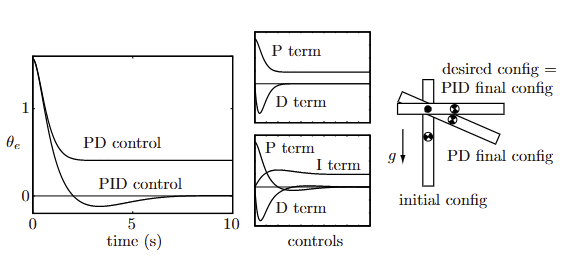
\includegraphics[width=0.8\linewidth]{img/pid.png}
\end{figure}


For basic flight stabilization where the full dynamic behavior of the plant is not realized, a simple PD action can provide satisfactory performance


\subsection{Attitude Control}

The error between the target orientation $q_{\text{target}}$ and the current body orientation $q_{\text{body}}$ is defined as:

$$\Delta q = q_{\text{target}} \cdot q_{\text{body}}^{-1}$$

Using Unity’s `ToAngleAxis` method, this relative rotation is converted into an angle $\phi$ and an axis $\mathbf{n}$. The error vector $\mathbf{e}$ is then:

$$\mathbf{e} = \phi \cdot \mathbf{n}$$

The controller applies a PD loop (Proportional-Derivative) to generate corrective torque.

$$\boldsymbol{\tau}_{\text{world}} = K_p \cdot \mathbf{e} + K_d \cdot \frac{\mathbf{e} - \mathbf{e}_{k-1}}{\Delta t}$$

Finally, the world-space torque is transformed into the body frame ($R_{\text{wb}}$) for the physics simulation:

$$\boldsymbol{\tau}_{\text{body}} = R_{\text{wb}} \cdot \boldsymbol{\tau}_{\text{world}}$$


\section{Drone Agent: A PID Implementation for Self-Leveling drones}

\subsection{Introduction to PID Control}

In 1922, Nicolas Minorsky presented a very clear analysis of the control actions necessary to provide effective control of a system whose exact dynamics were un- known. He analyzed the actions taken by a good helmsman steering a ship and translated these actions into the appropriate mathematical formulations \parencite{bennett1993pid}. It is now know as the Proportional-Integral-Derivative (PID) controller. PID is a type of controller that is most commonly used and applied in mechanical systems \parencite{idrissi_review_2022}.

The controller consists of three main components:

\begin{itemize}
    \item Proportional ($K_p$): Acts like a virtual spring that pulls the system toward the desired position; the control action increases as the error gets larger.
    \item Integral ($K_i$): Accumulates the error over time to eliminate steady-state error, ensuring the drone reaches the exact target even in the presence of disturbances like gravity.
    \item erivative ($K_d$): Acts as a virtual damper to reduce oscillations and prevent the system from overshooting its target.
\end{itemize}

The idealized control law is expressed as:

$$u(t) = K_p e(t) + K_i \int e(t) dt + K_d \frac{de(t)}{dt}$$

\subsection{Path Generation}

The objective of this chapter is to implement a closed-loop mission controller. This system translates high-level world-frame goals (waypoint coordinates, target altitude, and yaw) into RC-style stick commands (normalized -1 to 1) compatible with the existing Yue drone physics engine.

To move between points, the agent generates a path using two Cubic Bézier curves. Given four control points $P_0, P_1, P_2, P_3$, home to waypoint and back \cref{fig:path}, the position $B(t)$ for $t \in [0,1]$ is defined as:


$$B(t) = (1-t)^3 P_0 + 3(1-t)^2 t P_1 + 3(1-t) t^2 P_2 + t^3 P_3$$

\begin{figure}
    \caption{Path Design}
    \label{fig:path}
    \centering
    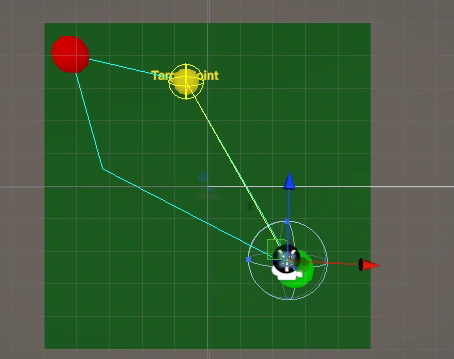
\includegraphics[width=0.8\linewidth]{img/path.png}
\end{figure}

The path is constructed relative to the "Home" ($P_{home}$) and "Target" ($P_{target}$) vectors:

\begin{itemize}
    \item Forward Vector: $\vec{f} = \text{normalize}(P_{target} - P_{home})$
    \item Orthogonal (Right) Vector: $\vec{r} = \vec{up} \times \vec{f}$ (This handles the lateral expansion of the teardrop).
    \item Bulge Parameterization: A `widthRatio` variable allows the path to scale from a narrow line to a wide teardrop shape.
\end{itemize}

The mission follows a two-phase approach to ensure a continuous loop:

\begin{itemize}
    \item Outbound: Path from Home to Waypoint using a right-hand offset for control points.
    \item Inbound: Path from Waypoint back to Home using a left-hand offset.
\end{itemize}

\subsubsection{ Cascaded Control Loops}

The system employs a cascaded control scheme where the Outer Loop (Position) provides setpoints for the Inner Loop (Attitude/Velocity).

\begin{itemize}
    \item The Inner Loop features controllers that yield the required rolling and pitching moments $\tau_x$ and $\tau_y$ to regulate horizontal movement. The Inner Loop block requires the current quadcopter attitude as well as reference signals for roll and pitch to obtain its output \parencite{paredes2021quadcopter}.
    \item The Outer Loop, which features controllers that yield the required thrust differential and yawing moments as well as the desired reference signals.
\end{itemize}

\subsection{Implementation Logic}

During takeoff, the controller focuses exclusively on vertical error ($e_y$). The vertical force $force_Y$ is mapped to a normalized throttle value ($T$):

$$T = \frac{u_T + 1}{2}$$

Following a path requires a look-ahead method. Given current position $\mathbf{p}$ and look-ahead target $\mathbf{t}$ on the path, the position error is defined as:

$$
e_x = t_x - p_x,\quad e_y = t_y - p_y,\quad e_z = t_z - p_z
$$

The Outer Loop converts this error into a Desired Velocity in the world axis:

$$v_{x,\text{des}} = \text{PID}_X(e_x),\quad v_{z,\text{des}} = \text{PID}_Z(e_z)$$

To translate these into drone-relative commands (Pitch/Roll), the world velocity is projected onto the drone's Heading Axis:

\begin{itemize}
    \item Forward Basis: $\hat{\mathbf{f}} = R_y(\psi)\,\hat{\mathbf{z}}_{\text{forward}}$
    \item Right Basis: $\hat{\mathbf{r}} = R_y(\psi)\,\hat{\mathbf{x}}_{\text{right}}$
    \item Projections:$$v^{\parallel}_{\text{des}} = \mathbf{v}_{H,\text{des}}\cdot\hat{\mathbf{f}}, \quad v^{\perp}_{\text{des}} = \mathbf{v}_{H,\text{des}}\cdot\hat{\mathbf{r}}$$
\end{itemize}

The Inner Loop then calculates the error between desired and actual velocity to produce stick inputs:

\begin{itemize}
    \item Pitch (Right Vertical): Based on longitudinal velocity error ($e_{v,\parallel}$).
    \item Roll (Right Horizontal): Based on lateral velocity error ($e_{v,\perp}$).
\end{itemize}


The drone should yaw toward its movement direction once a "velocity threshold" (0.5 m/s) is met.

\begin{itemize}
    \item Target Yaw: $\psi_{\text{target}} = \operatorname{atan2}(v_x,\,v_z)$
    \item Yaw Error: $e_\psi = \text{DeltaAngle}(\psi, \psi_{\text{target}})$
    \item Output: $u_{\text{yaw}} = \text{PID}_{\text{yaw}}(e_\psi)$
\end{itemize}


By calculating these normalized joystick rates, the system can visualize the "AI's intent" on the HUD. This serves as a co-training hinter, showing human pilots the optimal stick positions for maintaining the designated path \cref{fig:ui}.

\begin{figure}
    \caption{hinter UI}
    \label{fig:ui}
    \centering
    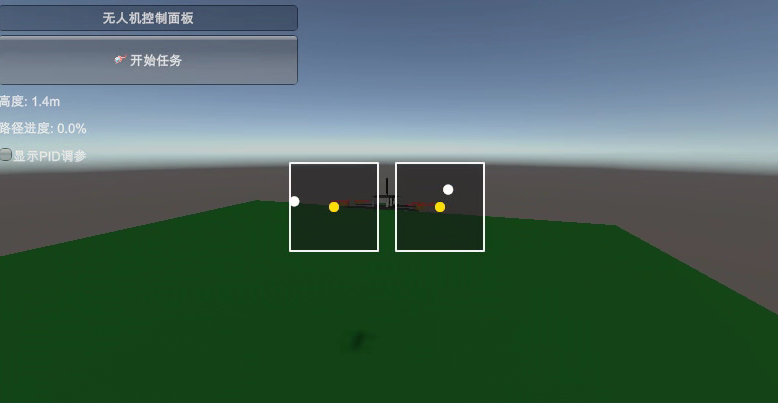
\includegraphics[width=0.8\linewidth]{img/ui.png}
\end{figure}

\subsection{Drone Agent: A RL Implementation for Self-Leveling drones}

While Proportional-Integral-Derivative (PID) controllers are the industry standard for stable piloting—offering a simple, "white-box" solution—they often struggle with complex, non-linear dynamics where the Integral term alone is insufficient. Recently, Reinforcement Learning (RL) has gained traction as a robust "black-box" alternative. To reduce the computational burden on onboard systems, reinforcement learning has increasingly been adopted as a key approach for autonomous obstacle avoidance (Yu et al., 2025).

While many RL solutions bridge the gap from computer vision to control, this chapter explores a "target-to-target" approach. Using Unity’s ML-Agents toolkit, I aim to develop a training pipeline that investigates the efficacy of RL for precise drone hovering.

\subsection{Fundamentals of Reinforcement Learning}

The concept of implementing RL in computing is among the earliest visions of AI. In a 1948 report, Alan Turing described a design for a pleasure-pain system (Barto, 2019). Modern RL defines a framework where an agent learns behavior through trial-and-error interactions with a dynamic environment (Kaelbling et al., 1996). Unlike supervised learning, the agent is not provided with "correct" answers. Instead, it receives a scalar reinforcement signal (reward or punishment) and must discover actions that maximize its long-term cumulative reward.

\subsubsection{Markov Decision Processes (MDPs)}

MDPs provide the mathematical foundation for RL \cref{fig:des}. In an MDP, an agent’s actions influence both the immediate reward and the subsequent state of the environment. An MDP is formally defined by:

\begin{itemize}
    \item A set of states (S): Possible environment configurations.
    \item A set of actions (A): Choices available to the agent.
    \item A reward function (R): $R: S \times A \to \mathbb{R}$, specifying the instantaneous reward.
    \item A state transition function (T): $T: S \times A \to \Delta(S)$, defining the probability of transitioning to state $s'$ given action $a$ in state $s$.
\end{itemize}

\begin{figure}
    \caption{Markov Decision Process diagram}
    \label{fig:des}
    \centering
    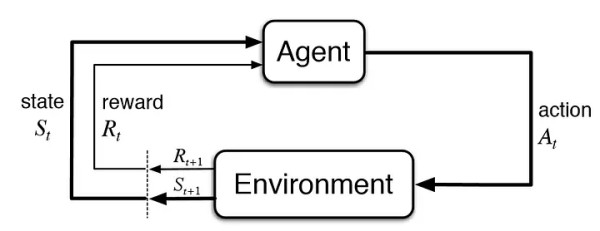
\includegraphics[width=0.8\linewidth]{img/decision.jpg}
\end{figure}

\subsection{Implementation with Unity ML-Agents}

ML-Agents \cref{fig:agent} enable games and simulations to serve as environments for training intelligent agents in Unity. Training can be done with reinforcement learning, imitation learning, neuroevolution, or any other methods. Trained agents can be used for many use cases, including controlling NPC behavior (in a variety of settings such as multi-agent and adversarial), automated testing of game builds and evaluating different game design decisions pre-release.

Every Learning Environment will always have one Agent for every character in the scene. While each Agent must be linked to a Behavior, it is possible for Agents that have similar observations and actions to have the same Behavior.

\begin{figure}
    \caption{Simplified ML-Agents Scene Block Diagram}
    \label{fig:agent}
    \centering
    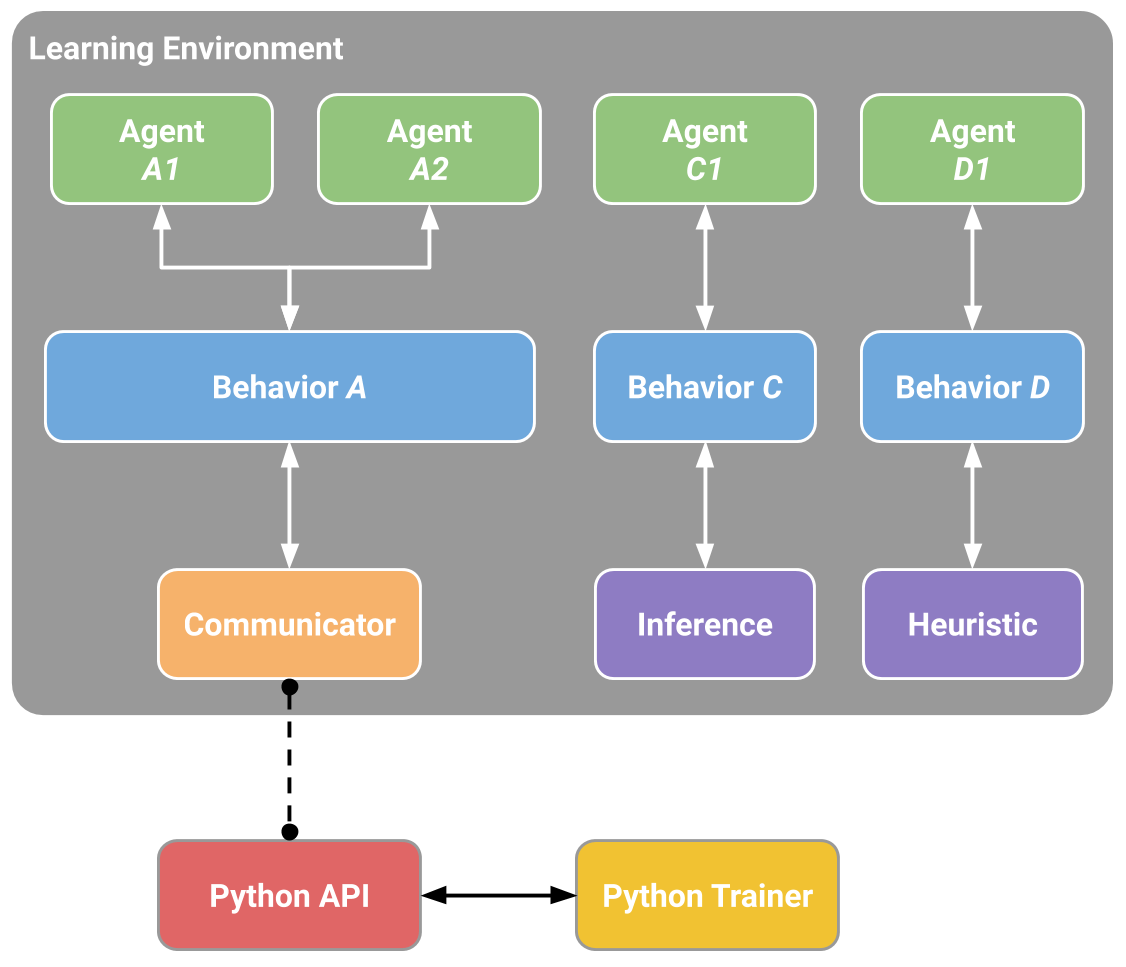
\includegraphics[width=0.8\linewidth]{img/agent.png}
\end{figure}

For this research, each Drone Agent includes:

\begin{itemize}
    \item Agent Script: Handles `OnActionReceived` (processing "joystick" inputs), `CollectObservations` (monitoring states), and `Heuristic` (manual control for debugging).
    \item Behavior Parameters: Defines the vector space for actions and observations.
    \item Decision Requester: Controls the frequency of actions. By limiting the request rate, we can simulate more "human-like" reaction times, making the agent a better tutor for human pilots.
\end{itemize}

\subsection{The Hovering Task}

We implemented a 1D control mission: regulating the drone's vertical position ($y$) within a target band $[H - R, H + R]$, where $H$ is the `targetHeight` and $R$ is the `acceptableRadius`.

The following two values are being observed.

\begin{itemize}
    \item Normalized Height Error: $\text{clip}(\frac{y - H}{R}, -k, k) / k$ (where $k$ is `errorClampK`). This maps the error to a $[-1, 1]$ range, preventing extreme spikes from destabilizing the gradient.
    \item Vertical Velocity: $v_y / v_{\text{ref}}$, clipped to $[-1, 1]$.
\end{itemize}

The agent uses one continuous action in the range $[0, 1]$, representing the throttle input.

Rewards are calculated at each decision step ($\Delta t$):

\begin{itemize}
    \item Event-based: A `firstArrivalReward` is granted upon entering the target band for the first time per episode.
    \item Dense/Steady-state: A `livingRewardPerSecond` is granted while maintaining position within the band.
    \item Shaping: A penalty proportional to the normalized excess $(|e|-R)/R$ is applied when outside the band to discourage drifting.
\end{itemize}

\subsection{Proximal Policy Optimization (PPO)}


We utilized Proximal Policy Optimization (PPO), an on-policy actor-critic algorithm that updates policies in small, clipped steps to ensure stability (OpenAI, 2017). PPO is particularly effective for drones learning to navigate complex environments (Yu et al., 2025).

The optimization objective is defined as:
$$L^{CLIP}(\theta) = \hat{\mathbb{E}}_t [ \min(r_t(\theta)\hat{A}_t, \text{text{clip}}(r_t(\theta), 1-\epsilon, 1+\epsilon)\hat{A}_t) ]$$


\begin{itemize}
    \item $\theta$ is the policy parameter
    \item $\hat{E}_t$ denotes the empirical expectation over timesteps
    \item $r_t$ is the ratio of the probability under the new and old policies, respectively
    \item $\hat{A}_t$ is the estimated advantage at time $t$
    \item $\epsilon$ is a hyperparameter, usually $0.1$ or $0.2$
\end{itemize}

The agent was trained for $5 \times 10^5$ steps using the following hyperparameters:

\begin{itemize}
    \item Clipping parameter $\epsilon = 0.2$
    \item GAE parameters $(\lambda, \gamma) = 0.99$
    \item Neural network: a 2-layer MLP with $128$ hidden units
    \item Learning rate: $3 \times 10^{-4}$ with linear decay
\end{itemize}

To monitor progress, we implemented a color-coded feedback system, \cref{fig:train}:

\begin{itemize}
    \item Yellow: Below target.
    \item Orange: Above target.
    \item Blue: Stable hovering.
\end{itemize}

\begin{figure}
    \caption{trainig process}
    \label{fig:train}
    \centering
    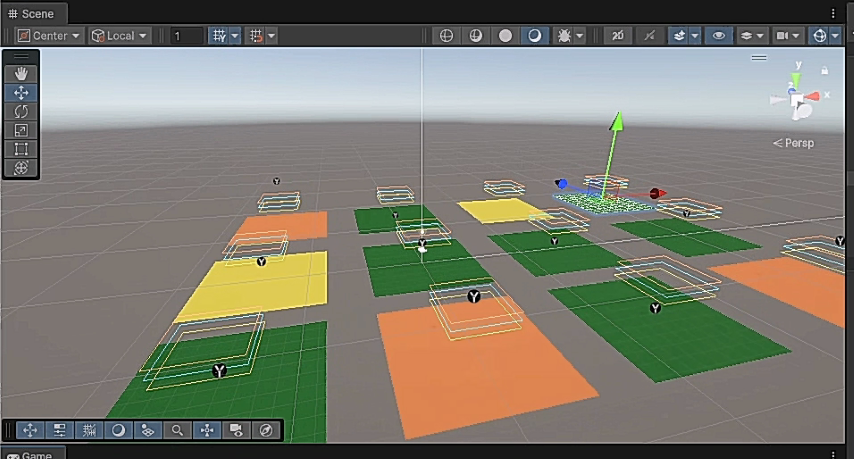
\includegraphics[width=0.8\linewidth]{img/train.png}
\end{figure}

Cumulative Reward: Showed steady growth after 100k steps, plateauing at 400k, \cref{fig:result}.

Episode Length: Positively correlated with rewards; as the agent improved, it survived longer without crashing (falling too low).

Environment/Cumulative Reward Histograms: also shows when training time raises, reward start to raise.

\begin{figure}
    \caption{Result}
    \label{fig:result}
    \centering
    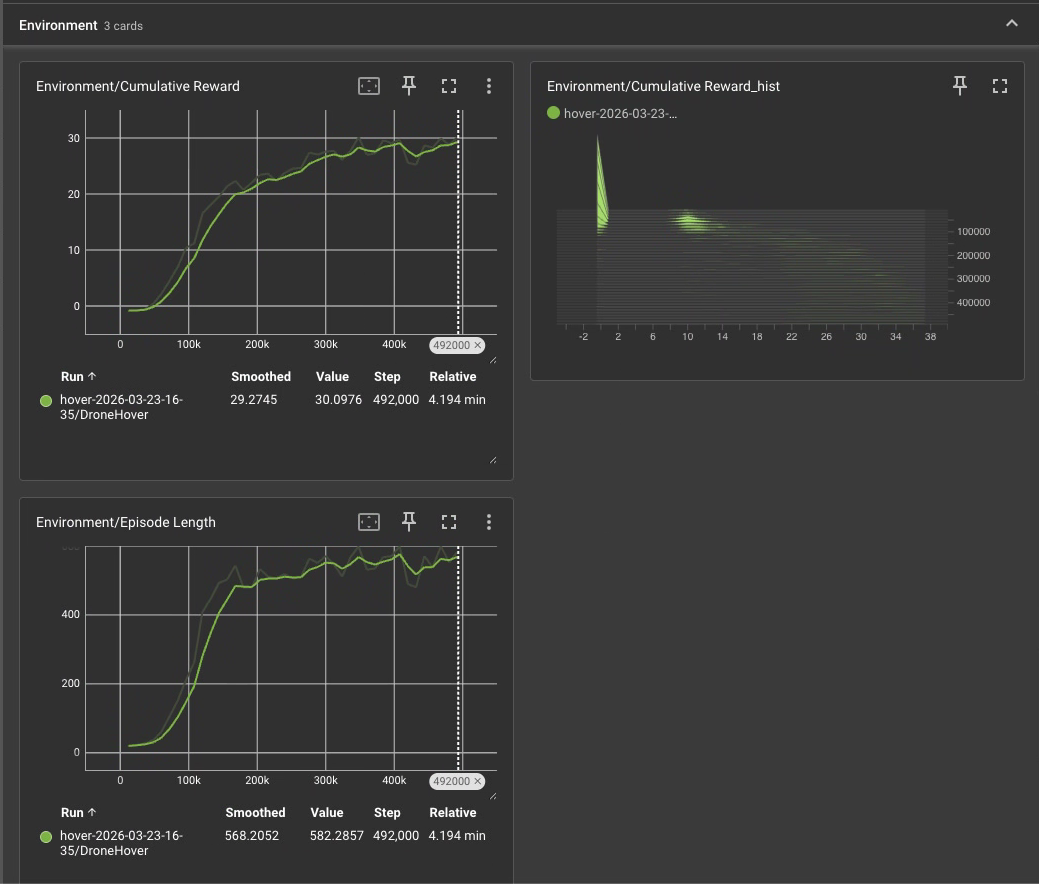
\includegraphics[width=0.8\linewidth]{img/result.png}
\end{figure}

\subsubsection{Tutoring UI}

The RL agent successfully learned to hover with high precision. By adjusting the `DecisionRequester`, we created a smoother control hint for the UI, matching the pace of human perception \cref{fig:hover}.

\begin{figure}
    \caption{Result}
    \label{fig:hover}
    \centering
    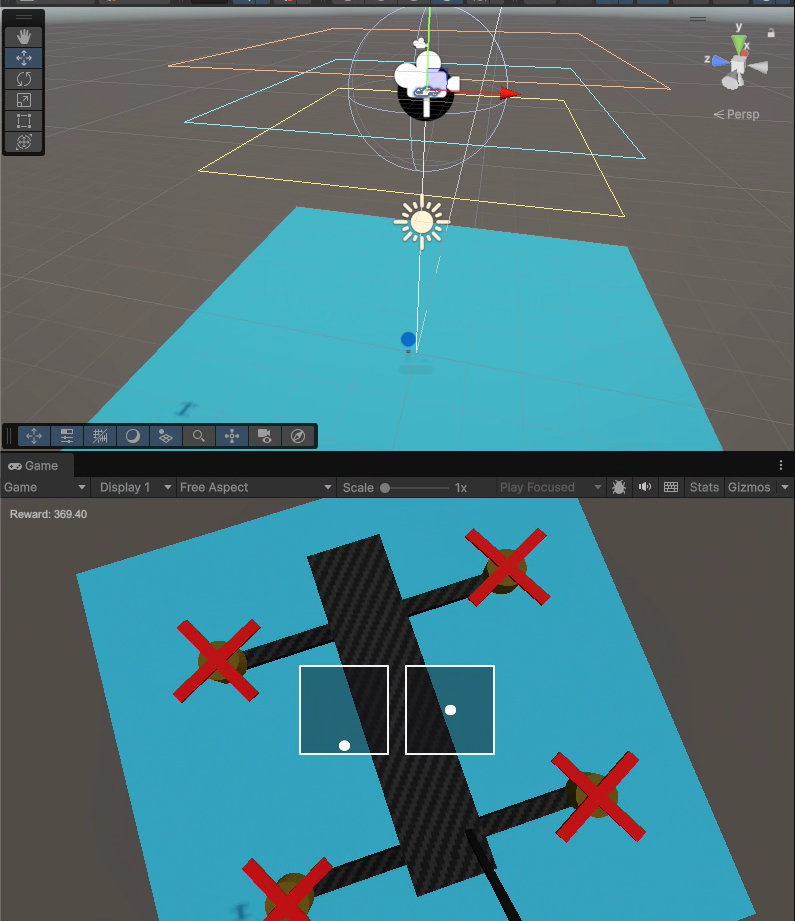
\includegraphics[width=0.8\linewidth]{img/hover.png}
\end{figure}

\section{Comparison of Current XR Development Platforms}

XR development is heavily dictated by the choice of game engine. Before initiating a project, it is critical to determine the target hardware and environmental requirements, as these factors define the development constraints.

Due to hardware availability, this paper focuses exclusively on development for the Meta Quest 3.

\subsubsection{Hardware Architectures: PC VR vs. Standalone}

For Head-Mounted Devices (HMDs) like the Meta Quest, two primary architectural configurations exist:

PC VR (Tethered): The headset acts as a peripheral. Assets are rendered on a high-end PC and streamed to the device via a wired (Link) or wireless (Air Link) connection. This allows developers to utilize the full power of engines like Unreal Engine, enabling high-fidelity features such as Lumen and Nanite. PC VR also supports specialized peripherals like haptic suits or omnidirectional treadmills, as seen in industry-standard titles like Half-Life: Alyx.

Standalone VR (All-in-One): Standalone headsets are self-contained systems with internal mobile chipsets. These provide high mobility but require significant optimization. High-end features must often be disabled or simplified to maintain performance. However, lightweight engines like Unity or Godot excel in this space, offering a balance between visual quality and mobile performance.

Rendevski et al. (2022) note that Standalone VR (SVR) applications offer significant advantages over PC VR. With proper optimization techniques, almost any PC VR scenario can be developed and deployed as SVR while still providing an acceptable user experience.

Differently, a recent survey from the Game Developers Conference (GDC) shows that among developers interested in creating VR/AR/MR games, the SteamVR platform (PC VR) slightly surpassed the Meta Quest / Horizon Store (68\% vs. 64\%) as their platform of interest. These were followed by PlayStation VR/VR2 (34\%) and Apple visionOS (15\%). However, when filtering for developers who have actually worked on VR/AR/MR games, a strong preference remains for the Meta Quest (72\%) over SteamVR (59\%).

\subsubsection{Passthrough (video see-through)}

Mixed reality (MR) headsets create immersive experiences designed to spatially integrate virtual content into the physical world. The newest headsets rely on passthrough video. While using passthrough, a person does not see light from the real world but instead relies on stereoscopic, color, high resolution, low latency, real-time video of the world, which is displayed on small screens inside a headset.(Bailenson et al., 2024)

Waldow et al. (2025) investigates Pass-Through Embodiment (PTE), The study found that PTE significantly enhances the user’s sense of presence and embodiment compared to using a customizable digital avatar. The ability to see one’s own body strengthens the feeling of being physically "present" in the VR environment without negatively affecting performance or causing sickness.

Leveraging passthrough on modern XR devices can help developers build highly engaging mixed-reality environments, which is particularly beneficial for applications like prototyping drone simulations.

\subsubsection{Software Standards}

To ensure cross-platform compatibility, developers rely on unified industry standards. Currently, there are two major public standards:

- OpenXR
- WebXR

\subsubsection{OpenXR}


OpenXR is the industry-standard API for XR applications. It is the interface between an application and an in-process or out-of-process “XR runtime system”. The runtime system handles functionality such as frame composition, peripheral management, and raw tracking information (Khronos OpenXR Working Group, 2024). Major game engines and the Meta Spatial SDK are built upon OpenXR to ensure hardware-agnostic development.

A primary bottleneck in XR development is the "deployment loop." Compiling a standalone APK and pushing it to a device can take 10–15 minutes per iteration.

- Link Mode: Developers often use the Oculus Link App to preview scenes in PC VR, though this requires constantly putting on and taking off the headset.

- Simulators: The Meta XR Simulator is increasingly becoming the preferred method for rapid iteration, allowing developers to simulate head and controller movements directly on their PC without needing physical hardware.

\subsubsection{WebXR}

The WebXR Device API provides the interfaces necessary to enable developers to build compelling, comfortable, and safe immersive applications on the web across a wide variety of hardware form factors (World Wide Web Consortium, 2022).

WebXR serves as a higher-level abstraction that runs in the browser, combining older specifications from WebVR and WebAR. The WebXR standard shares core features with and can be viewed as a subset of OpenXR.

While traditional game engines offer WebXR export support, there are fewer dedicated development stacks built exclusively for it. This section focuses specifically on engines that directly call the browser API.

For security reasons, WebXR APIs are restricted to HTTPS. Consequently, developers must use port-forwarding technologies during local development. Thanks to the efficiency of the web stack, a WebXR application typically only requires a few seconds to bundle. It is worth noting, however, that web rendering technology is currently transitioning from WebGL2 to WebGPU, which may introduce API changes in the WebXR ecosystem.


\subsubsection{Software Engine Comparison}

\begin{table}[h]
\centering
\begin{tabular}{l|l|l|l|l}
\hline
Feature & Unreal Engine (5.7) & Unity (6.0) & Godot (4.6) & Wonderland Engine \\
\hline
Primary Language & C++ / Blueprints & C\# & GDScript / C\# / C++ & JavaScript / TypeScript \\
Physics Engine & Chaos Physics & NVIDIA PhysX / DOTS & Jolt Physics (Integrated) & NVIDIA PhysX \\
Rendering Tech & Lumen (Dynamic GI) \& Nanite (Virtual Geometry) & URP / HDRP & Forward+ / Mobile & WebGL2 \\
Meta Support & Fork build & First-class Support & Community-driven (GDExtension) & No support \\
Machine Learning Support & Learning Agent & ML Agents & Godot RL Agents & No support \\
Editor Size (XR plugin included) & $\sim$50GB+ & $\sim$20GB & $<1$GB & 200MB \\
\hline
\end{tabular}
\caption{Comparison of game engines}
\end{table}

- Unreal Engine: UE is known for photorealistic rendering, UE provides unparalleled visual fidelity. Its Chaos Physics engine is highly regarded for complex simulations, making it the foundation for projects like Microsoft’s AirSim. However, UE has a high barrier to entry: the editor is massive, and utilizing Meta’s private APIs often requires compiling a custom engine branch from source.

- Unity: Unity remains the most popular choice for Meta Quest development due to its mature SDK support and C\# scripting. While it uses PhysX by default, its DOTS (Data-Oriented Technology Stack) provides high-performance physics for complex drone swarms. It offers the most streamlined "out-of-the-box" experience for Standalone VR.

- Godot: Godot has emerged as a powerful, lightweight alternative. It is highly compatible with modern AI coding assistants due to its Python-like GDScript. The integration of Jolt Physics as the default 3D engine has resolved previous performance hurdles for VR. However, its XR ecosystem is largely community-maintained. While excellent for prototyping, the lack of official Meta API support and the potential instability of third-party GDExtensions require careful dependency management for production-grade projects.

- Wonderland Engine: Wonderland Engine is a specialized WebXR engine built in C++ and compiled to WebAssembly.  By leveraging WebGL2, it achieves the performance necessary to render thousands of objects at native frame rates directly within a browser. . The development workflow relies on JavaScript and TypeScript, providing a highly familiar and accessible environment for traditional web developers. A unique advantage is the ability to edit scenes directly on the headset, enabling instant feedback without removing the device.





